\section{Implementation}
\label{implementation}

The heart of the implementation is to implement a set of mutation-testing operators
so that a mutation-based fuzzer can apply them to
inputs.  There is a large literature on the selection of mutation
operators for mutation testing, but this literature focuses on identifying
operators that help find holes in a testing effort.  There is no
reason to believe that this is particularly indicative of the
operators that will be most useful in fuzzing, and there is some
suggestion that such approaches do not outperform random selection in any case~\cite{MutReduct}.  We therefore 
used a large number of operators that apply to a wide variety of
programming languages, based on the set of operators provided by the
Universal Mutator tool.

\subsection{Fast or Smart?}

More important than the selection of the best mutation operators
(which will likely vary considerably by target compiler) is a
fundamental decision.  A mutation testing tool can be highly intelligent, only
applying operators in ways that should produce compiling code, based
on a parse of the program to be mutated.  Or, like the Universal
Mutator, it can be ``dumb'' and apply rules without expensive analysis
of the code, trusting a compiler to prune invalid
mutants.  Which approach is best for fuzzing is not obvious: on the
one hand, all fuzzing (including generative) relies on executing very
large numbers of inputs; most ``random'' inputs will be uninteresting,
neither exposing a bug nor novel behavior to drive further
exploration.  Fuzzer throughput is a critical factor, and a ``dumb''
mutation strategy can produce modified inputs much more rapidly than a
``smart'' approach that must parse the input.  On the other hand, if a
shallower analysis during mutation production greatly decreases the
probability that the mutated inputs will expose bugs or new behavior,
the result is, effectively, slower fuzzing.  If adding a parsing stage
makes mutation generation take twice as long, but more than doubles
the probability the input generated will be useful, it will be a net
gain for in-practice fuzzing throughput.

Of course, at first
glance, it would appear that  ``smart'' strategies are not even
possible for us: there will often not be a parser that the
tool could use.  However, as we discuss below, recent work on
multi-language syntax transformation~\cite{combypaper} enables an approach that can use
\emph{syntax fragments} to provide a significant degree of intelligent
mutation without specialized parsers for a compiler's input language,
at the cost of additonal time required to synthesize inputs.

\begin{sloppypar}
\subsubsection{Fast String-level Approximation of Mutation Operators}
\label{strat-fast-string-level}

\begin{figure}[h!]
\begin{lstlisting}[basicstyle=\scriptsize\ttfamily,numbers=none,xleftmargin=0.7em,xrightmargin=.7em]
case (?{\color{blu}0}?): (?{\color{dkgreen}/* Semantic statement deletion */}?)
  strncpy(original, (?{\color{dkred}\verb|"\n"|}?), MAX_MUTANT_CHANGE);
  strncpy(replacement, (?{\color{dkred}\verb|"\nif (0==1)\n"|}?), MAX_MUTANT_CHANGE);
  break;
case (?{\color{blu}1}?):
  strncpy(original, (?{\color{dkred}\verb|"("|}?), MAX_MUTANT_CHANGE);
  strncpy(replacement, (?{\color{dkred}\verb|"(!"|}?), MAX_MUTANT_CHANGE);
  break;
(?{\color{blu}\textbf{\texttt{...}}?)
case (?{\color{blu}53}?): (?{\color{dkgreen}/* Swap comma delimited things case 4 */}?)
 delim_swap(out_buf, temp_len, &original, 
            &replacement, pos, (?{\color{dkred}\verb|","|}?), (?{\color{dkred}\verb|","|}?), (?{\color{dkred}\verb|")"|}?));
  break;
case (?{\color{blu}54}?): (?{\color{dkgreen}/* Just delete a line */?)
  delim_replace(out_buf, temp_len, &original, 
                &replacement, pos, (?{\color{dkred}\verb|"\n"|}?), (?{\color{dkred}\verb|"\n"|}?), (?{\color{dkred}\verb|""|}?));
  break;
case (?{\color{blu}55}?): (?{\color{dkgreen}/* Delete something like "const" case 1 */}?)
  delim_replace(out_buf, temp_len, &original, 
                &replacement, pos, (?{\color{dkred}\verb|" "|}?), (?{\color{dkred}\verb|" "|}?), (?{\color{dkred}\verb|""|}?));
  break;    
\end{lstlisting}
\caption{Part of the Fast String-Based Approximation}
\label{fig:foperators}
\end{figure}

The core implementation of our technique is a text-based approximation
of the regular expression based approach taken by the Universal
Mutator.  Rather than call the mutation tool, which is written in
Python and relatively slow, we hand-crafted, using low-level C string
libraries, approximations of the mutation operators for all languages
(the ``universal'' rules from the universal mutator) and those for
``C-like'' languages.  Figure \ref{fig:foperators} shows part of the
implementation.  Most operators are implemented by choosing a string
to find and a string to replace it with; the mutator finds a random
occurrence of the {\tt original} string and replaces it with the {\tt
  replacement} string.  Other operators require more involved string
manipulation, e.g., removing a semicolon-delimited statement, or
swapping function arguments.  Critically, however, all operations
involve only basic C string operations, and no more than 4 linear
scans of the entire text to be mutated.  The vast majority of operations require no
more than one linear scan in the worst case, and most scans terminate
before scanning a large fragment of the input.  When an operation that
is chosen cannot be applied (e.g., the string to be replaced is not
present), another operation is attempted, up to a maximum number of
tries.

\end{sloppypar}

This approach is, as stated, fast.  While slower than many built-in
AFL mutations (obviously searching for strings is slower than flipping
a randomly chosen bit, or incrementing a byte value), it has a fairly
low upper bound on worst-case runtime, and very good average runtime.  The time required is much
closer to AFL's built in mutations than to techniques such as
solving constraints, even a linear
approximation~\cite{Eclipser}, and is successful much, much, more
often than solving constraints over compiler inputs, which are among
the hardest conceivable for modern SMT solvers or linear
approximations to handle.  Figure \ref{fig:fopexample} shows some
sample transformations of inputs using this approach.  Notice that
some of the mutations tend to delete code, potentially large amounts
of code.  This is critical for enabling the fuzzer engine to compose
interesting inputs, in that the larger two inputs are, the
more likely they will have, e.g., namespace conflicts that prevent
merging them.

\begin{figure}[h!]
\begin{subfigure}{.65\columnwidth}
\begin{lstlisting}[basicstyle=\scriptsize\ttfamily,numbers=none,xleftmargin=0.7em,xrightmargin=.7em]
...
 int bar(int x, int y, int z) {
   if (x < y)
     return foo(x, y, z);
   while (x < y) {
     x++;
     z = z * 2;
   }
}
\end{lstlisting}
\subcaption{Original code}
\end{subfigure}
%%%%%%%%%%%%%%%%%%%%%%%%%%%%%%%%%%%%%%%%%%%%%%%%%%%%%%%%%%%%%%%%%%%%%%%%%%%%%%%%%%%%%%%%%%%%%%%%%%%%
\begin{subfigure}{.45\columnwidth}
\begin{lstlisting}[basicstyle=\scriptsize\ttfamily,numbers=none,xleftmargin=0.7em,xrightmargin=.7em]
...
 if (x (?{\color{dkred}\textbf{\texttt{==}}}?) y)
   return foo(x, y, z);
\end{lstlisting}
\end{subfigure}
\hspace{.2em}
\begin{subfigure}{.45\columnwidth}
\begin{lstlisting}[basicstyle=\scriptsize\ttfamily,numbers=none,xleftmargin=0.7em,xrightmargin=.7em]
...
 if (x (?{\color{dkred}\textbf{\texttt{<}}}?) y)
   return foo(x, z, y);
\end{lstlisting}
\end{subfigure}
\begin{subfigure}{.45\columnwidth}
\begin{lstlisting}[basicstyle=\scriptsize\ttfamily,numbers=none,xleftmargin=0.7em,xrightmargin=.7em]
...
 while (x < y) {
   x++;
   (?{\color{dkred}break;}?)
\end{lstlisting}
\end{subfigure}
\hspace{.2em}
\begin{subfigure}{.45\columnwidth}
\begin{lstlisting}[basicstyle=\scriptsize\ttfamily,numbers=none,xleftmargin=0.7em,xrightmargin=.7em]
...
 while (x < y) {
   x++; 
 }
\end{lstlisting}
\end{subfigure}
\subcaption{Four mutations}
\label{fig:fopexample}
\caption*{\normalsize\textbf{Figure 3.} Mutations of  Simple Code} % HACK: hardcoded figure so that subcpations work, don't know how to override subcaptions.
\end{figure}

\subsubsection{Smart Syntax-Aware Mutation}
\label{strat-syntax-aware}

\begin{sloppypar}
Our core approach uses fast mutation written in C that we added directly to
AFL's fuzzing hot loop. Our early success with this method prompted us to
augment AFL further with even smarter mutations to find more bugs more quickly.
The intuition behind these smarter mutations is to manipulate (typically
larger) code fragments that are likely to be syntactically valid and yet
trigger deeper buggy properties (past compiler parsing). Unlike transformtions
in the core approach that approximate syntactically valid transformations on
strings or lines, syntax-aware transformations seek to accurately modify syntax
in well-parenthesized expressions or entire multiline code blocks (e.g.,
function or \texttt{for}-loop bodies). In general, manipulating a program's
parse tree like this imposes exactly the kind of burden and complexity that
small compiler projects can't support (defining a precise grammar, keeping
tooling up to date as the grammar evolves). Even with multi-year investment in
tools, effort necessarily goes into deeper focus on
language-specific properties and semantics %, rather than broad, language-general approaches.
that may not generalize to other compilers.
\end{sloppypar}

\begin{sloppypar}
Our approach combats this cost by using the
\texttt{Comby}\footnote{\href{https://comby.dev}{https://comby.dev}} tool~\cite{combypaper} to do
syntax-aware code matching and transformation. \texttt{Comby} works by coarsely
parsing a program, taking care to correctly interpret nested syntax of code
(parentheses and braces), and avoids conflating this syntax with strings and
comments, as regular expressions (and our string approach) tends to do.  \texttt{Comby} is not a fully-fledged
parser for any language, but it \emph{is} language-aware, in that it recognizes
a small set of language-specific constructs (e.g., syntax to identify quoted
strings or comments) to accurately parse code blocks. \texttt{Comby} supports
over 50 languages, and uses a generic parser for unsupported languages like custom
DSLs. \texttt{Comby} is likely to perform ``well-enough'' for any language
anyone is likely to want to input to a compiler.
\end{sloppypar}

\texttt{Comby} does not have C bindings, so we expose its transformation
abilities as a server to our AFL fuzzer. We implemented a minimal HTTP client
in the fuzzer's hot loop to request inputs. We use the \texttt{Comby} server in
a mutation mode where it \emph{generates} inputs from a decomposition of
\emph{templates} and \emph{concrete fragments} obtained from the initial corpus
of programs. We first preprocess all programs in the initial corpus to obtain
this decomposition. The following figure illustrates the decomposition of an
example Zig program.

\begin{figure}[h!]
\begin{subfigure}{\columnwidth}
\begin{lstlisting}[basicstyle=\scriptsize\ttfamily,numbers=none,xleftmargin=1em,xrightmargin=14em]
function f(uint256 arg) public {
    f(notfound);
}
\end{lstlisting}
\vspace{-1em}
\end{subfigure}
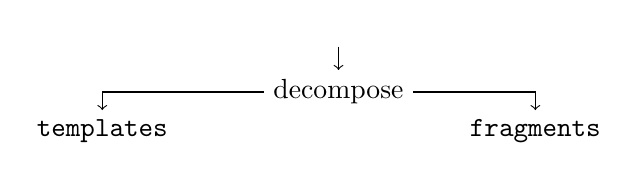
\begin{tikzpicture}[node distance=2cm]
% nodes
\node (Q) at (3, 1.2) {};
\node (C) at (3, .5) {decompose};
\node (A) at (0, 0) {\tt templates};
\node (D) at (5.5, 0) {\tt fragments};

% arrows
\draw[->] (Q) edge (C);
\draw[->, to path={-| (\tikztotarget)}]
  (C) edge (A)
  (C) edge (D);
\end{tikzpicture}
\end{figure}

\begin{figure}[h!]
\vspace{-2.0em}
\begin{subfigure}{.64\columnwidth}
\begin{lstlisting}[basicstyle=\scriptsize\ttfamily,numbers=none,xleftmargin=0.7em,xrightmargin=0em]
function f(uint256 arg) public {(?{\color{dkgreen}\$1}?)}
\end{lstlisting}
\end{subfigure}\hspace{.5em}
\begin{subfigure}{.26\columnwidth}
\begin{lstlisting}[basicstyle=\scriptsize\ttfamily,numbers=none,xleftmargin=0.7em,xrightmargin=0em]
f(notfound);
\end{lstlisting}
\end{subfigure}

\begin{subfigure}{.64\columnwidth}
\begin{lstlisting}[basicstyle=\scriptsize\ttfamily,numbers=none,xleftmargin=0.7em,xrightmargin=0em]
function f((?{\color{dkgreen}\$1}?)) public {
    f(notfound);
} 
\end{lstlisting}
\end{subfigure}\hspace{.5em}
\begin{subfigure}{.26\columnwidth}
\begin{lstlisting}[basicstyle=\scriptsize\ttfamily,numbers=none,xleftmargin=0.7em,xrightmargin=0em]
uint256 arg
\end{lstlisting}
\vspace{1.5em}
\end{subfigure}

\begin{subfigure}{.64\columnwidth}
\begin{lstlisting}[basicstyle=\scriptsize\ttfamily,numbers=none,xleftmargin=0.7em,xrightmargin=0em]
function f(uint256 arg) public {
    f((?{\color{dkgreen}\$1}?));
} 
\end{lstlisting}
\end{subfigure}\hspace{.5em}
\begin{subfigure}{.26\columnwidth}
\begin{lstlisting}[basicstyle=\scriptsize\ttfamily,numbers=none,xleftmargin=0.7em,xrightmargin=0em]
notfound
\end{lstlisting}
\vspace{1.5em}
\end{subfigure}
\end{figure}

A ``decompose'' operation yields three \texttt{templates} in the left column
({\tt\color{dkgreen}\$1} are placeholders for future substitution) and extracts
three corresponding concrete \texttt{fragments}, shown in the right column. 
The ``decompose'' operation is done with \texttt{Comby}, which extracts concrete
values inside parentheses, braces, and square brackets (patterns
\texttt{(\$expr)}, \texttt{\{\$expr\}}, \texttt{[\$expr]} respectively). Note
that our approach can be customized to extract \emph{any} kind of syntactically
significant pattern and correspondingly decompose the input program; we simply
chose syntax that commonly delineates code blocks and expressions (i.e.,
parentheses and braces) since these exhibit interesting properties that
preserve structure (multiline statements, well-formed expressions) that go
beyond what string-level mutations identify.

We perform this decomposition for all programs in the corpus to obtain
templates and concrete fragments, which we then deduplicate. Once fuzzing, the
server generates an input program by selecting, uniformly at random, a template
and up to 10 program fragments and then substitutes all locations in the
template with program fragments. In essence, the server splices new inputs that
are likely to compose syntactically well-formed programs.

In addition to generating inputs, the server can also apply syntax-aware
\texttt{Comby} transformation rules, analogous to string-level mutation
operators. In practice, our server architecture adds considerable overhead (we
discuss this in Section~\ref{eval}) and is thus slow in applying
on-the-fly mutations, and in that sense less
appealing than the string-level mutation. Our
results in Section~\ref{eval} do show, however, that generative
syntax-aware input manipulation demonstrates compelling utility despite
incurring significant slowdown.\footnote{We are actively improving the tooling
architecture, a matter of engineering rather than
limitations on the inherent merits of the approach.}

\subsubsection{P(havoc) + P(text) + P(splice) = 1}

Our full implementation is based on Google's released code for the AFL
fuzzer, and available as an open source tool (that, to date, has 68
stars on GitHub, has been forked 7 times, and has external users who
make bug reports and queries to us).\footnote{Link omitted for
  blinding.}  The main change to AFL is the addition of code such as that shown in
Figure~\ref{fig:foperators}.  The new version (the ``AFL compiler
fuzzer'') can also call out to {\tt comby} to generate mutants.  Two
new command line parameters to AFL control the use of these features:
{\tt -1} determines the probability to generate a mutant using the
fast C string implementation (with a default value of 75\%), and {\tt -2} determines the probability
to call {\tt comby} to generate a mutant (with a default value of
0\%).  If these two parameters add up to less than 100\%, the
remainder of the time the usual stock AFL havoc mutation operators are
applied; by default, this happens 25\% of the time.
